\EXERCISE
در شکل زیر یک شبکه مربعی 
$11 \times 6$
نمایش داده شده است . در این شکل 
$4$
 پاره خط 
$AB, CD, EF, GH$
  مشخص شده‌اند . تعداد کوچکترین مسیرهایی را که از 
$O$
  به 
$P$
   می‌روند را در هر یک از
حالات زیر بدست آورید.

الف) از هیچ‌ کدام از این خط‌ها عبور نکند.

ب) هر مسیر از دقیقا دو پاره خط از آن‌ها عبور کند.

    \begin{center}
     	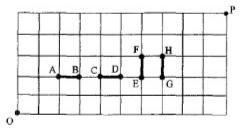
\includegraphics[scale=0.7]{./5.png}
    \end{center}